\section{Tools: Dynamic Programming, Continuous-Time Stochastic Processes, Markov Chains}

This section collects the mathematical tools used throughout the course: (i) dynamic programming in continuous time (the Hamilton--Jacobi--Bellman, or HJB, equation), with and without uncertainty; (ii) the Kolmogorov forward equation for the evolution of a distribution; (iii) Brownian motion and its relatives; (iv) It\^o's lemma; (v) discrete Markov chains.

%=====================================================================
\subsection{Overview: three forms of the HJB equation \pg{11--12}}

\paragraph{Notation used in this subsection.}
\begin{itemize}
\item $t$: time (continuous); $T$: terminal date ($T=\infty$ for an infinite horizon).
\item $x$: \emph{state variable} (e.g.\ wealth or capital). It is given at each instant and can only be changed gradually.
\item $u$: \emph{control variable} (e.g.\ consumption). The agent chooses it at each instant.
\item $f(x,u,t)$: flow return (instantaneous payoff, e.g.\ utility of consumption).
\item $g(x,u,t)$: law of motion of the state, $\dot x\equiv dx/dt=g(x,u,t)$ (e.g.\ the budget constraint).
\item $\rho>0$: subjective discount rate.
\item $V$: value function, the maximal attainable value of the objective starting from a given state (and date). Subscripts denote partial derivatives: $V_t=\partial V/\partial t$, $V_x=\partial V/\partial x$, $V_{xx}=\partial^2V/\partial x^2$; $V'(x)$ is the ordinary derivative when $V$ depends on $x$ only.
\item $W_t$: standard Brownian motion (defined in Section~\ref{sec:sbm}); $dW_t$ is its increment.
\item $\mu(x,u)$, $\sigma(x)$: drift and volatility of the state when it is stochastic, $dx=\mu(x,u)\,dt+\sigma(x)\,dW$.
\end{itemize}

\begin{keybox}[title=Three forms of the HJB equation]
\begin{itemize}
\item \textbf{Classic HJB} (deterministic, time-dependent, typically finite horizon; a partial differential equation (PDE) in $(x,t)$):
\begin{equation}\label{eq:hjb-classic}
-V_t(x,t)=\max_u\big\{f(x,u,t)+V_x(x,t)\,g(x,u,t)\big\}.
\end{equation}
\item \textbf{Stationary HJB} (deterministic, infinite horizon, time enters only through discounting at rate $\rho$; an ordinary differential equation (ODE) in $x$ only):
\begin{equation}\label{eq:hjb-stat}
\rho V(x)=\max_u\big\{f(x,u)+V'(x)\,g(x,u)\big\}.
\end{equation}
\item \textbf{Stochastic HJB} (state follows $dx=\mu(x,u)\,dt+\sigma(x)\,dW$; a second-order ODE):
\begin{equation}\label{eq:hjb-stoch}
\rho V(x)=\max_u\Big\{f(x,u)+V_x(x)\,\mu(x,u)+\tfrac12\sigma^2(x)V_{xx}(x)\Big\}.
\end{equation}
\end{itemize}
\end{keybox}

How to read the differences:
\begin{itemize}
\item \textbf{Finite horizon / time-dependent problem.} The value changes with calendar time, and this is captured by $V_t$ on the left-hand side. Any discounting is written inside $f$ (e.g.\ $f=e^{-\rho t}u(c)$), so there is no separate $\rho V$ term. Look at $f$ to decide whether the factor $e^{-\rho t}$ must be written in.
\item \textbf{Infinite horizon, stationary problem.} Calendar time no longer matters (the future always looks the same from the current state), so $V$ depends on $x$ only and discounting appears as the term $\rho V$.
\item \textbf{Deterministic vs.\ stochastic.} Deterministic DP has no $dW$ term. Stochastic DP $=$ deterministic DP $+$ It\^o's lemma: randomness adds the second-order term $\tfrac12\sigma^2V_{xx}$.
\end{itemize}
The three equations are derived step by step below.

%=====================================================================
\subsection{Deterministic dynamic programming and the classic HJB \pg{11--12}}

\paragraph{Setup.} The generic deterministic problem is
\begin{equation}\label{eq:ddp-problem}
\max_{\{u_t\}}\int_0^T f(x_t,u_t,t)\,dt\qquad\text{s.t.}\qquad \dot x_t=g(x_t,u_t,t),\quad x_0\ \text{given}.
\end{equation}
Example: $x$ = wealth, $u$ = consumption, $\dot x=g$ is the budget constraint (how wealth changes given income and spending).

\paragraph{Key assumptions.} Dynamic programming works because the problem can be split into ``what happens now'' and ``the continuation problem from tomorrow on''. This requires:
\begin{enumerate}
\item Today's action affects current and future returns, but not past returns.
\item Current returns depend on current and past actions (through the state), but not on future actions.
\end{enumerate}
Under these assumptions, the value from date $t$ onward depends only on the current state $x$ and date $t$:
\[
V(x,t)=\max_{\{u_s\}_{s\ge t}}\int_t^T f(x_s,u_s,s)\,ds\quad\text{s.t. } \dot x_s=g(x_s,u_s,s),\ x_t=x.
\]

\paragraph{Derivation of the classic HJB from the Bellman equation.}
Split the interval $[t,T]$ into a short first piece $[t,t+\Delta t]$ and the rest. Over the short piece the agent picks $u$ and earns approximately $f(x,u,t)\,\Delta t$; after it, the agent is at state $x+\Delta x$ at date $t+\Delta t$ and behaves optimally, earning $V(x+\Delta x,t+\Delta t)$. This gives the \emph{Bellman equation}
\begin{align*}
V(x,t)&=\max_u\Big\{f(x,u,t)\,\Delta t+V(x+\Delta x,\,t+\Delta t)\Big\},\qquad \Delta x\approx g(x,u,t)\,\Delta t.
\intertext{First-order Taylor expansion of the continuation value around $(x,t)$:}
V(x+\Delta x,t+\Delta t)&\approx V(x,t)+V_x(x,t)\,g(x,u,t)\,\Delta t+V_t(x,t)\,\Delta t.
\intertext{Substitute into the Bellman equation:}
V(x,t)&=\max_u\Big\{f(x,u,t)\,\Delta t+V(x,t)+V_x\,g(x,u,t)\,\Delta t+V_t\,\Delta t\Big\}.
\intertext{Subtract $V(x,t)$ from both sides ($V$ does not depend on $u$, so it can be taken out of the max):}
0&=\max_u\Big\{f(x,u,t)\,\Delta t+V_x\,g(x,u,t)\,\Delta t\Big\}+V_t\,\Delta t.
\intertext{Divide by $\Delta t$ and let $\Delta t\to0$ (the approximation errors are of order $(\Delta t)^2$ and vanish):}
-V_t(x,t)&=\max_u\Big\{f(x,u,t)+V_x(x,t)\,g(x,u,t)\Big\},
\end{align*}
which is \eqref{eq:hjb-classic}. The first-order condition (FOC) of the maximisation is $f_u+V_x\,g_u=0$: the marginal flow return of the control equals the marginal loss in continuation value. $V_x$ is the \emph{shadow price} of the state (the value of one more unit of $x$).

%---------------------------------------------------------------------
\subsubsection{Worked example: consumption with CRRA utility and a linear budget constraint}

\paragraph{Setup.}
\begin{itemize}
\item $c_t\ge0$: consumption (control); $k_t$: capital / the ``cake'' (state), $k_0$ given.
\item Utility: CRRA, $u(c)=\dfrac{c^{1-\gamma}}{1-\gamma}$, with $\gamma>0$, $\gamma\ne1$ = coefficient of relative risk aversion ($1/\gamma$ = elasticity of intertemporal substitution). Marginal utility is $u'(c)=c^{-\gamma}$.
\item Discount rate $\rho>0$; infinite horizon.
\item Law of motion (continuous time): $\dot k_t=a\,k_t-c_t$, where $a$ is the constant net rate of return on the stock. Cases: $a=0$ is pure cake eating (then $\int_0^\infty c_t\,dt=k_0$); $a=-\delta$ is a cake that depreciates at rate $\delta$; $a=A-\delta$ is the AK model with depreciation.
\end{itemize}
The problem is
\begin{equation}\label{eq:cake-problem}
\max_{\{c_t\}}\int_0^\infty e^{-\rho t}\,\frac{c_t^{1-\gamma}}{1-\gamma}\,dt\qquad\text{s.t.}\qquad \dot k_t=a\,k_t-c_t,\quad k_0\ \text{given}.
\end{equation}
We solve it with the classic HJB, keeping the factor $e^{-\rho t}$ inside $f$ (so $f(k,c,t)=e^{-\rho t}c^{1-\gamma}/(1-\gamma)$, $g(k,c)=ak-c$).

\paragraph{Step 1: HJB.} From \eqref{eq:hjb-classic},
\begin{equation}\label{eq:cake-hjb}
-V_t(k,t)=\max_c\Big\{e^{-\rho t}\frac{c^{1-\gamma}}{1-\gamma}+V_k(k,t)\,(ak-c)\Big\}.
\end{equation}

\paragraph{Step 2: FOC.} Differentiate the bracket with respect to $c$ and set to zero:
\begin{align}
e^{-\rho t}c^{-\gamma}-V_k&=0\notag\\
\Longrightarrow\quad e^{-\rho t}c^{-\gamma}&=V_k\qquad\text{(discounted marginal utility = shadow price of capital)}\notag\\
\Longrightarrow\quad c^{-\gamma}&=V_k\,e^{\rho t}\qquad\text{(multiply by $e^{\rho t}$)}\notag\\
\Longrightarrow\quad c^*&=\big(V_k\,e^{\rho t}\big)^{-1/\gamma}\qquad\text{(raise to the power $-1/\gamma$).}\label{eq:cake-foc}
\end{align}
Plugging \eqref{eq:cake-foc} back into \eqref{eq:cake-hjb} gives a PDE in $V$ alone:
\[
-V_t=e^{-\rho t}\frac{\big(V_ke^{\rho t}\big)^{-\frac{1-\gamma}{\gamma}}}{1-\gamma}+V_k\Big(ak-\big(V_ke^{\rho t}\big)^{-1/\gamma}\Big).
\]

\paragraph{Step 3: Guess.} Because utility is CRRA and the constraint is linear, guess a value function of the same power form:
\begin{equation}\label{eq:cake-guess}
V(k,t)=B\,e^{-\rho t}\,\frac{k^{1-\gamma}}{1-\gamma},\qquad B>0\ \text{an unknown constant}.
\end{equation}
Its derivatives are
\begin{align*}
V_t&=-\rho B\,e^{-\rho t}\frac{k^{1-\gamma}}{1-\gamma}\qquad\text{(derivative of $e^{-\rho t}$ is $-\rho e^{-\rho t}$)},\\
V_k&=B\,e^{-\rho t}k^{-\gamma}\qquad\text{(derivative of $k^{1-\gamma}/(1-\gamma)$ is $k^{-\gamma}$)}.
\end{align*}

\paragraph{Step 4: Consumption rule implied by the guess.} Insert $V_k$ into \eqref{eq:cake-foc}:
\begin{align*}
c^*&=\big(B\,e^{-\rho t}k^{-\gamma}\,e^{\rho t}\big)^{-1/\gamma}=\big(B\,k^{-\gamma}\big)^{-1/\gamma}=B^{-1/\gamma}\,k.
\end{align*}
Define $\theta\equiv B^{-1/\gamma}$, so $c^*=\theta k$: consumption is a constant fraction $\theta$ of capital. A useful identity: $\theta^{1-\gamma}=\theta\cdot\theta^{-\gamma}=\theta B$.

\paragraph{Step 5: Substitute into the HJB and solve for $B$.}
Each term of \eqref{eq:cake-hjb}, evaluated at $c^*=\theta k$:
\begin{align*}
-V_t&=\rho B\,e^{-\rho t}\frac{k^{1-\gamma}}{1-\gamma},\\
e^{-\rho t}\frac{(c^*)^{1-\gamma}}{1-\gamma}&=e^{-\rho t}\frac{\theta^{1-\gamma}k^{1-\gamma}}{1-\gamma}=B\,e^{-\rho t}\frac{\theta\,k^{1-\gamma}}{1-\gamma}\quad\text{(using $\theta^{1-\gamma}=\theta B$)},\\
V_k\,(ak-c^*)&=B\,e^{-\rho t}k^{-\gamma}(a-\theta)k=B\,e^{-\rho t}(a-\theta)\,k^{1-\gamma}.
\end{align*}
So the HJB becomes
\[
\rho B\,e^{-\rho t}\frac{k^{1-\gamma}}{1-\gamma}=B\,e^{-\rho t}\frac{\theta\,k^{1-\gamma}}{1-\gamma}+B\,e^{-\rho t}(a-\theta)\,k^{1-\gamma}.
\]
Divide both sides by $B\,e^{-\rho t}k^{1-\gamma}$ (this is where the guess is verified: $k$ and $t$ drop out, so the guess works if a constant $\theta$ solves what is left):
\begin{align*}
\frac{\rho}{1-\gamma}&=\frac{\theta}{1-\gamma}+a-\theta\\
\frac{\rho}{1-\gamma}&=\theta\Big(\frac{1}{1-\gamma}-1\Big)+a=\frac{\gamma}{1-\gamma}\,\theta+a\qquad\text{(collect $\theta$ terms)}\\
\rho&=\gamma\,\theta+(1-\gamma)a\qquad\text{(multiply by $1-\gamma$)}\\
\theta&=\frac{\rho-(1-\gamma)a}{\gamma}.
\end{align*}
Finally $B=\theta^{-\gamma}$.

\begin{keybox}[title={Solution of the deterministic CRRA problem}]
\[
\frac{c^*}{k}=\theta=\frac{\rho-(1-\gamma)a}{\gamma},\qquad B=\Big(\frac{\rho-(1-\gamma)a}{\gamma}\Big)^{-\gamma},\qquad V(k,t)=B\,e^{-\rho t}\frac{k^{1-\gamma}}{1-\gamma}.
\]
We need $\theta>0$, i.e.\ $\rho>(1-\gamma)a$; this guarantees that utility is finite and the transversality condition $\lim_{t\to\infty}e^{-\rho t}V_k k_t=0$ holds (no capital is left unused ``at infinity'').
For the depreciating-cake form $\dot k=(1-\delta)k-c$ set $a=1-\delta$: $B=\big(\frac{\rho+(\gamma-1)(1-\delta)}{\gamma}\big)^{-\gamma}$.
\end{keybox}

\paragraph{Interpretation.}
\begin{itemize}
\item Capital grows at $\dot k/k=a-\theta=\dfrac{a-\rho}{\gamma}$, and since $c=\theta k$, consumption grows at the same rate. This is the usual Euler equation $\dot c/c=(r-\rho)/\gamma$ with $r=a$.
\item $\partial\theta/\partial a=-(1-\gamma)/\gamma$: a higher return lowers the consumption share if $\gamma<1$ (substitution effect dominates: save more) and raises it if $\gamma>1$ (income effect dominates). With log utility ($\gamma\to1$) $\theta=\rho$, independent of $a$.
\end{itemize}

\begin{tipbox}
Recipe for guess-and-verify: write the HJB $\to$ take the FOC $\to$ guess $V$ of the same functional form as utility $\to$ compute $V_t,V_k$ (and $V_{kk}$ if stochastic) $\to$ substitute into the HJB $\to$ divide out $k$ and $t$ $\to$ solve for the constant $\to$ recover $c^*$.
\end{tipbox}

%=====================================================================
\subsection{The stationary HJB (infinite horizon) \pg{12}}

\paragraph{Setup.} Infinite horizon, flow return $e^{-\rho t}f(x,u)$ where $f$ does not depend on $t$, and law of motion $\dot x=g(x,u)$ that does not depend on $t$:
\[
\max_{\{u_t\}}\int_0^\infty e^{-\rho t}f(x_t,u_t)\,dt\quad\text{s.t.}\quad \dot x_t=g(x_t,u_t),\ x_0\ \text{given}.
\]
Define the \emph{current-value} value function $V(x)$ = maximal value of $\int_t^\infty e^{-\rho(s-t)}f\,ds$ starting from $x_t=x$. Because the problem looks identical at every date, $V$ does not depend on $t$.

\paragraph{Derivation (from the discounted Bellman equation).}
\begin{align*}
V(x)&=\max_u\Big\{f(x,u)\,\Delta t+e^{-\rho\Delta t}\,V(x+\Delta x)\Big\},\qquad \Delta x\approx g(x,u)\,\Delta t.
\intertext{Use $e^{-\rho\Delta t}\approx1-\rho\Delta t$ and $V(x+\Delta x)\approx V(x)+V'(x)g(x,u)\Delta t$:}
V(x)&=\max_u\Big\{f\,\Delta t+(1-\rho\Delta t)\big(V(x)+V'(x)g\,\Delta t\big)\Big\}\\
&=\max_u\Big\{f\,\Delta t+V(x)+V'(x)g\,\Delta t-\rho V(x)\Delta t-\rho V'(x)g\,(\Delta t)^2\Big\}.
\intertext{Subtract $V(x)$, divide by $\Delta t$, let $\Delta t\to0$ (the $(\Delta t)^2$ term vanishes):}
\rho V(x)&=\max_u\Big\{f(x,u)+V'(x)\,g(x,u)\Big\},
\end{align*}
which is \eqref{eq:hjb-stat}. It is an ODE: only derivatives with respect to the single variable $x$ appear.

\paragraph{Link to the classic HJB.} Writing the present-value function as $\tilde V(x,t)=e^{-\rho t}V(x)$ in \eqref{eq:hjb-classic} gives $\tilde V_t=-\rho e^{-\rho t}V$ and $\tilde V_x=e^{-\rho t}V'$; dividing the classic HJB by $e^{-\rho t}$ yields exactly \eqref{eq:hjb-stat}. This is why the factor $e^{-\rho t}$ is \emph{absent} from the flow return in a stationary HJB: it was divided out in this step. (In the example above, $V(k,t)=e^{-\rho t}\cdot B k^{1-\gamma}/(1-\gamma)$ has precisely this form.)

\begin{keybox}[title=Asset-pricing interpretation]
\[
\underbrace{\rho V(x)}_{\text{required (riskless) return}}=\underbrace{f(x,u)}_{\text{dividend}}+\underbrace{V'(x)\,g(x,u)}_{\text{capital gain }=dV/dt}.
\]
\end{keybox}
Think of $V$ as the price of an asset that pays the flow $f$. Holding it must earn the riskless return $\rho V$, which comes from the dividend plus the change in the asset's value as the state moves ($dV/dt=V'(x)\dot x$, chain rule).

%=====================================================================
\subsection{Stochastic dynamic programming: the stochastic AK model \pg{12--13}}

\paragraph{Derivation of the stochastic HJB.} Let the state follow $dx=\mu(x,u)\,dt+\sigma(x)\,dW$ (a diffusion; see Section~\ref{sec:diffusions}). The Bellman equation now has an expectation, because tomorrow's state is random:
\begin{align*}
V(x)&=\max_u\Big\{f(x,u)\,\Delta t+e^{-\rho\Delta t}\,\mathbb{E}\big[V(x+\Delta x)\big]\Big\}.
\intertext{By It\^o's lemma (Section~\ref{sec:ito}), $\mathbb{E}[V(x+\Delta x)]\approx V(x)+\big(V'(x)\mu(x,u)+\tfrac12\sigma^2(x)V''(x)\big)\Delta t$, because the $dW$ term has mean zero and $(\Delta x)^2\approx\sigma^2\Delta t$. Repeating the steps of the stationary case:}
\rho V(x)&=\max_u\Big\{f(x,u)+V_x\,\mu(x,u)+\tfrac12\sigma^2(x)V_{xx}\Big\},
\end{align*}
which is \eqref{eq:hjb-stoch}: \emph{SDP $=$ deterministic DP $+$ It\^o's lemma}. It is a second-order ODE (the time-dependent version would be a PDE). The expectation in the objective is fully captured by the extra term $\tfrac12\sigma^2V_{xx}$; no $\mathbb{E}$ and no $e^{-\rho t}$ remain in the equation.

%---------------------------------------------------------------------
\subsubsection{Example: the stochastic AK growth model}

\paragraph{Setup.}
\begin{itemize}
\item $k_t$: capital (state); $c_t$: consumption (control).
\item Technology: output $=Ak$ with constant productivity $A>0$ (no depreciation, or $A$ is net of depreciation).
\item Shocks: capital is hit by multiplicative (proportional) shocks of volatility $\sigma>0$; $W_t$ is a standard Brownian motion.
\item Preferences: CRRA with risk aversion $\gamma>0$, $\gamma\ne1$, discount rate $\rho$.
\end{itemize}
The household solves
\begin{equation}\label{eq:sak-problem}
\max_{\{c_t\}}\ \mathbb{E}_0\int_0^\infty e^{-\rho t}\frac{c_t^{1-\gamma}}{1-\gamma}\,dt\qquad\text{s.t.}\qquad dk_t=(Ak_t-c_t)\,dt+\sigma k_t\,dW_t.
\end{equation}
So the drift is $\mu(k,c)=Ak-c$ and the volatility is $\sigma(k)=\sigma k$; thus $\sigma(k)^2=\sigma^2k^2$.

\paragraph{Step 1: Stationary stochastic HJB.} Applying \eqref{eq:hjb-stoch}:
\begin{equation}\label{eq:sak-hjb}
\rho V(k)=\max_c\Big\{\frac{c^{1-\gamma}}{1-\gamma}+V_k\,(Ak-c)+\tfrac12\sigma^2k^2\,V_{kk}\Big\}.
\end{equation}

\paragraph{Step 2: FOC.} Differentiate with respect to $c$: $c^{-\gamma}-V_k=0$, so
\begin{equation}\label{eq:sak-foc}
c^*=V_k^{-1/\gamma}.
\end{equation}

\paragraph{Step 3: Guess.} $V(k)=B\,\dfrac{k^{1-\gamma}}{1-\gamma}$ (letter $B$ to avoid a clash with productivity $A$; no $e^{-\rho t}$ because the HJB is stationary). Then
\[
V_k=B\,k^{-\gamma},\qquad V_{kk}=-\gamma B\,k^{-\gamma-1}.
\]
From \eqref{eq:sak-foc}: $c^*=(Bk^{-\gamma})^{-1/\gamma}=B^{-1/\gamma}k\equiv\theta k$, and again $\theta^{1-\gamma}=\theta B$.

\paragraph{Step 4: Substitute into \eqref{eq:sak-hjb}.} Term by term:
\begin{align*}
\frac{(c^*)^{1-\gamma}}{1-\gamma}&=\frac{\theta^{1-\gamma}k^{1-\gamma}}{1-\gamma}=\frac{B\theta\,k^{1-\gamma}}{1-\gamma},\\
V_k(Ak-c^*)&=Bk^{-\gamma}(A-\theta)k=B(A-\theta)\,k^{1-\gamma},\\
\tfrac12\sigma^2k^2V_{kk}&=\tfrac12\sigma^2k^2\big(-\gamma Bk^{-\gamma-1}\big)=-\tfrac12\gamma\sigma^2B\,k^{1-\gamma}.
\end{align*}
Hence
\[
\rho B\frac{k^{1-\gamma}}{1-\gamma}=\frac{B\theta\,k^{1-\gamma}}{1-\gamma}+B(A-\theta)k^{1-\gamma}-\tfrac12\gamma\sigma^2B\,k^{1-\gamma}.
\]
\paragraph{Step 5: Solve for $\theta$.} Divide by $Bk^{1-\gamma}$:
\begin{align*}
\frac{\rho}{1-\gamma}&=\frac{\theta}{1-\gamma}+A-\theta-\frac{\gamma\sigma^2}{2}\\
&=\frac{\gamma}{1-\gamma}\theta+A-\frac{\gamma\sigma^2}{2}\qquad\text{(collect $\theta$ terms as before)}\\
\rho&=\gamma\theta+(1-\gamma)\Big(A-\frac{\gamma\sigma^2}{2}\Big)\qquad\text{(multiply by $1-\gamma$)}\\
\theta&=\frac{\rho-(1-\gamma)\big(A-\tfrac12\gamma\sigma^2\big)}{\gamma}.
\end{align*}

\begin{keybox}[title=Stochastic AK model: consumption rule]
\[
\frac{c^*}{k}=\theta=B^{-1/\gamma}=\frac{\rho-(1-\gamma)\big(A-\tfrac12\gamma\sigma^2\big)}{\gamma},\qquad V(k)=\theta^{-\gamma}\frac{k^{1-\gamma}}{1-\gamma}.
\]
Capital follows $dk=(A-\theta)k\,dt+\sigma k\,dW$ (a geometric Brownian motion), with expected growth rate $A-\theta$.
With $\sigma=0$ this collapses to the deterministic solution with $a=A$.
\end{keybox}
\paragraph{Interpretation.} Risk enters exactly like a reduction of the return from $A$ to the \emph{certainty-equivalent return} $A-\tfrac12\gamma\sigma^2$: the more risk-averse the household ($\gamma$) and the riskier capital ($\sigma$), the lower the risk-adjusted return. Since $\partial\theta/\partial\sigma^2=-(1-\gamma)/2$, more risk acts like a lower return: it raises the consumption share when $\gamma>1$ (income effect dominates) and lowers it, i.e.\ raises saving, when $\gamma<1$ (substitution effect dominates). This mirrors the effect of $a$ in the deterministic case.

%=====================================================================
\subsection{Kolmogorov forward (Fokker--Planck) equation \pg{13}}

\paragraph{Setup.} $x_t$ follows the diffusion $dx=\mu(x)\,dt+\sigma(x)\,dW_t$. Let $g(x,t)$ be the probability density of $x$ across the population (or across possible realisations) at date $t$, with initial density $g(x,0)$ given. Notation: $g_t=\partial g/\partial t$.

\begin{keybox}[title={Kolmogorov forward equation (KFE, also called Fokker--Planck, KFP)}]
\begin{equation}\label{eq:kfe}
g_t(x,t)=-\frac{\partial}{\partial x}\big(\mu(x)\,g(x,t)\big)+\frac12\frac{\partial^2}{\partial x^2}\big(\sigma^2(x)\,g(x,t)\big).
\end{equation}
\end{keybox}
\begin{itemize}
\item First term: the drift transports mass (it shifts the density in the direction of $\mu$). Second term: the volatility spreads the density out.
\item \textbf{Stationary distribution:} set $g_t=0$ and solve the resulting ODE in $x$. This is how the stationary wealth distribution is obtained in Huggett/Aiyagari-type models in continuous time.
\item A unique solution is pinned down by the normalisation (boundary) condition $\int_{-\infty}^{\infty}g(x,t)\,dx=1$ (plus $g\to0$ at the boundaries).
\end{itemize}

\paragraph{Moments.} Once $g(x,t)$ is known, the expectation of any function $f$ is
\[
\mathbb{E}[f(x_t)]=\int f(x)\,g(x,t)\,dx,
\]
so, differentiating under the integral and using \eqref{eq:kfe},
\begin{equation}\label{eq:kfe-moment}
\frac{d\,\mathbb{E}[f(x_t)]}{dt}=\int f(x)\,g_t(x,t)\,dx=\int f(x)\Big[-\frac{\partial}{\partial x}\big(\mu g\big)+\frac12\frac{\partial^2}{\partial x^2}\big(\sigma^2g\big)\Big]dx.
\end{equation}
Integrating by parts (once for the first term, twice for the second; boundary terms vanish because $g\to0$) gives the equivalent form
\[
\frac{d\,\mathbb{E}[f(x_t)]}{dt}=\mathbb{E}\Big[\mu(x_t)f'(x_t)+\tfrac12\sigma^2(x_t)f''(x_t)\Big],
\]
which is exactly the expected drift of $f(x_t)$ from It\^o's lemma. Example: $f(x)=x$ gives $d\,\mathbb{E}[x_t]/dt=\mathbb{E}[\mu(x_t)]$.

\paragraph{Application: stationary distribution of an Ornstein--Uhlenbeck process.} Take $\mu(x)=\kappa(\bar x-x)$, $\sigma(x)=\sigma$ (see Section~\ref{sec:diffusions}). Set $g_t=0$ in \eqref{eq:kfe}:
\begin{align*}
0&=-\frac{d}{dx}\big(\mu g\big)+\frac{\sigma^2}{2}\frac{d^2g}{dx^2}=\frac{d}{dx}\Big[-\mu g+\frac{\sigma^2}{2}g'\Big].
\intertext{So the bracket (the probability flux) is constant; it must be zero since $g,g'\to0$ at $\pm\infty$:}
\frac{g'}{g}&=\frac{2\mu(x)}{\sigma^2}=\frac{2\kappa(\bar x-x)}{\sigma^2}.
\intertext{Integrate ($\int g'/g\,dx=\ln g$):}
\ln g(x)&=-\frac{\kappa}{\sigma^2}(x-\bar x)^2+\text{const}\quad\Longrightarrow\quad g(x)\propto\exp\Big(-\frac{(x-\bar x)^2}{2\,\sigma^2/(2\kappa)}\Big).
\end{align*}
So the stationary distribution is $N\big(\bar x,\ \sigma^2/(2\kappa)\big)$: centred at the long-run mean, and tighter when mean reversion $\kappa$ is strong relative to the shock volatility $\sigma$.

%=====================================================================
\subsection{From a random walk to Brownian motion: the binomial tree \pg{14}}

\paragraph{Discrete random walk.} $x_t=x_{t-1}+\varepsilon_t$ with $\varepsilon_t\overset{iid}{\sim}N(0,1)$. Iterating forward,
\[
x_{t+T}=x_t+\sum_{j=1}^{T}\varepsilon_{t+j}.
\]
\paragraph{Three properties we want to carry into continuous time.}
\begin{enumerate}
\item $\mathbb{E}(x_{t+1}\mid x_t)=x_t$: $x$ is a \emph{martingale}; the best forecast of tomorrow is today, i.e.\ no trend/no drift. (Because $\mathbb{E}\varepsilon_{t+1}=0$.)
\item $\operatorname{Var}(x_{t+\tau}\mid x_t)=\tau$: the conditional variance grows linearly with the horizon. (Sum of $\tau$ independent unit-variance shocks.)
\item The conditional distribution of $x_{t+1}$ given the information set $\mathcal F_t$ (everything known at $t$) is Gaussian.
\end{enumerate}

\paragraph{Binomial tree.} Divide time into small steps of length $\Delta t$. In each step, $x$ moves up or down by a fixed amount $\Delta h$:
\[
x_{t+\Delta t}=x_t+\varepsilon_{t+\Delta t},\qquad \varepsilon=\begin{cases}+\Delta h&\text{with probability }p,\\-\Delta h&\text{with probability }q=1-p.\end{cases}
\]

\begin{center}
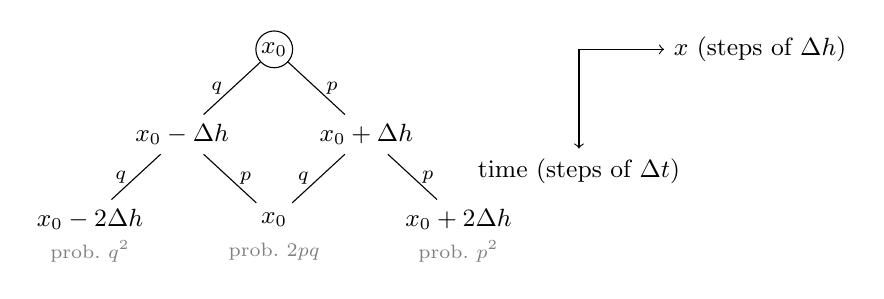
\begin{tikzpicture}[scale=0.9,every node/.style={font=\small}]
\node[draw,circle,inner sep=1pt] (a) at (0,0) {$x_0$};
\node (b1) at (-1.3,-1.2) {$x_0-\Delta h$}; \node (b2) at (1.3,-1.2) {$x_0+\Delta h$};
\node (c1) at (-2.6,-2.4) {$x_0-2\Delta h$}; \node (c2) at (0,-2.4) {$x_0$}; \node (c3) at (2.6,-2.4) {$x_0+2\Delta h$};
\draw (a)--node[left,font=\scriptsize]{$q$}(b1); \draw (a)--node[right,font=\scriptsize]{$p$}(b2);
\draw (b1)--node[left,font=\scriptsize]{$q$}(c1); \draw (b1)--node[right,font=\scriptsize]{$p$}(c2);
\draw (b2)--node[left,font=\scriptsize]{$q$}(c2); \draw (b2)--node[right,font=\scriptsize]{$p$}(c3);
\node[gray,font=\scriptsize] at (-2.6,-2.85) {prob.\ $q^2$};
\node[gray,font=\scriptsize] at (0,-2.85) {prob.\ $2pq$};
\node[gray,font=\scriptsize] at (2.6,-2.85) {prob.\ $p^2$};
\draw[->] (4.3,0)--(5.5,0) node[right]{$x$ (steps of $\Delta h$)};
\draw[->] (4.3,0)--(4.3,-1.4) node[below]{time (steps of $\Delta t$)};
\end{tikzpicture}
\end{center}
\textit{How to read the figure.} Time runs downward, one row per step $\Delta t$; the horizontal position is the value of $x$. From each node the process goes right (up by $\Delta h$) with probability $p$ or left (down by $\Delta h$) with probability $q$. The tree recombines (up-then-down and down-then-up both return to $x_0$), so after two steps the probabilities of the three possible values are $q^2$, $2pq$, $p^2$.

\paragraph{Moments of one step.}
\begin{align*}
\mathbb{E}[\Delta x]&=p\,\Delta h+q\,(-\Delta h)=(p-q)\,\Delta h,\\
\mathbb{E}[(\Delta x)^2]&=p\,(\Delta h)^2+q\,(\Delta h)^2=(\Delta h)^2.
\end{align*}
\paragraph{Choosing the step size.} Set $p=q=\tfrac12$ (no drift, property 1) and $\Delta h=\sigma\sqrt{\Delta t}$, so that $(\Delta h)^2/\Delta t=\sigma^2$. Over a horizon $T$ there are $n=T/\Delta t$ independent steps, so
\[
\operatorname{Var}(x_T-x_0)=n\,(\Delta h)^2=\frac{T}{\Delta t}\,\sigma^2\Delta t=\sigma^2T\qquad(=T\text{ when }\sigma=1),
\]
which is property 2. As $\Delta t\to0$, $x_T-x_0$ is a sum of many iid steps, so by the central limit theorem it becomes Gaussian (property 3).

\begin{tipbox}
The step must scale with $\sqrt{\Delta t}$, not $\Delta t$. If $\Delta h\propto\Delta t$, the variance $\frac{T}{\Delta t}(\Delta h)^2\propto T\Delta t\to0$ and the limit is deterministic; if $\Delta h$ shrinks more slowly than $\sqrt{\Delta t}$ the variance explodes. Only $\Delta h=\sigma\sqrt{\Delta t}$ gives a finite, non-zero variance per unit of time.
\end{tipbox}

%=====================================================================
\subsection{Brownian motion and diffusions \pg{14--16}}

\subsubsection{Standard Brownian motion (SBM)}\label{sec:sbm}
The limit of the binomial tree with $\sigma=1$ is the \emph{standard Brownian motion} $W_t$ (also called a Wiener process). It is a continuous-time Markov process with the following features:
\begin{enumerate}
\item \textbf{Continuous sample paths} (no jumps).
\item \textbf{Nowhere differentiable:} over a step, $\dfrac{\Delta x}{\Delta t}\sim\dfrac{\Delta h}{\Delta t}=\dfrac{\sigma\sqrt{\Delta t}}{\Delta t}=\dfrac{\sigma}{\sqrt{\Delta t}}\to\infty$ as $\Delta t\to0$. Hence $dW/dt$ does not exist; we always work with the increment $dW$ instead.
\item \textbf{Stationary, independent increments:} increments over non-overlapping intervals are independent, and their distribution depends only on the length of the interval.
\item \textbf{Mean zero, variance equal to elapsed time:} $W(0)=0$, $W(t)\sim N(0,t)$, and $W(t)-W(s)\sim N(0,t-s)$ for $s<t$.
\end{enumerate}

\paragraph{Increments.} For any discrete interval $\Delta t$,
\[
\Delta W_t=\varepsilon_t\sqrt{\Delta t},\qquad \varepsilon_t\sim N(0,1)\ \text{iid}.
\]
As $\Delta t\to0$, $dW=\varepsilon\sqrt{dt}$, and
\begin{align*}
\mathbb{E}[dW]&=\mathbb{E}[\varepsilon]\sqrt{dt}=0,\\
\mathbb{E}[(dW)^2]&=\mathbb{E}[\varepsilon^2]\,dt=dt\qquad(\text{since }\mathbb{E}[\varepsilon^2]=\operatorname{Var}\varepsilon=1).
\end{align*}
So $dW\sim N(0,dt)$, and summing increments, $W_t-W_s\sim N(0,t-s)$. Moreover $(dW)^2$ is of order $dt$ (not $dt^2$), which is why second-order terms survive in It\^o's lemma; in the limit one treats $(dW)^2=dt$ as non-random.

\paragraph{$p$-th variation.} For a partition $0=t_0<t_1<\dots<t_n=T$,
\[
V^p=\lim_{\max_k\Delta t_k\to0}\ \sum_{k=1}^n\big|x_{t_k}-x_{t_{k-1}}\big|^p.
\]
For SBM on $[0,T]$: each increment has size of order $\sqrt{\Delta t}$ and there are $T/\Delta t$ of them, so the sum is of order $\frac{T}{\Delta t}(\Delta t)^{p/2}$:
\begin{itemize}
\item $p=1$: order $T/\sqrt{\Delta t}\to\infty$, so $V^1=\infty$ (paths have infinite length; another sign of non-differentiability);
\item $p=2$: order $T$, and in fact $V^2=T$ exactly (\emph{quadratic variation} = elapsed time; this is the integrated form of $(dW)^2=dt$);
\item $p>2$: order $T(\Delta t)^{p/2-1}\to0$, so $V^p=0$.
\end{itemize}

\subsubsection{General (arithmetic) Brownian motion and diffusions}\label{sec:diffusions}
\begin{itemize}
\item \textbf{General (arithmetic) BM.} Build it from SBM by adding a drift $\mu$ and a volatility $\sigma$ (both constants):
\[
x_t=x_0+\mu t+\sigma W_t\qquad\Longleftrightarrow\qquad dx_t=\mu\,dt+\sigma\,dW_t.
\]
The second form is a \emph{stochastic differential equation} (SDE). Then $x_t-x_s\sim N\big(\mu(t-s),\ \sigma^2(t-s)\big)$.
\item \textbf{General diffusion.} Let drift and volatility depend on the state and time:
\[
dx_t=\underbrace{\mu(x,t)\,dt}_{\text{drift}}+\underbrace{\sigma(x,t)\,dW_t}_{\text{diffusion (random fluctuation)}}.
\]
By choosing $\mu(\cdot)$ and $\sigma(\cdot)$ one can generate almost any continuous-time stochastic process with continuous paths. Two important special cases follow.
\end{itemize}

\paragraph{Ornstein--Uhlenbeck (OU) process.} $\mu(x)=\kappa(\bar x-x)$ with $\kappa>0$, $\sigma(x,t)=\sigma$:
\begin{equation}\label{eq:ou}
dx_t=\kappa(\bar x-x_t)\,dt+\sigma\,dW_t.
\end{equation}
\begin{itemize}
\item $\bar x$: long-run mean; $\kappa$: speed of mean reversion (how fast $x$ is pulled back to $\bar x$).
\item When $x>\bar x$ the drift is negative, and when $x<\bar x$ it is positive, so $x$ is always pushed toward $\bar x$.
\item Taking expectations of \eqref{eq:ou} ($\mathbb{E}\,dW=0$): $\frac{d}{dt}\mathbb{E}[x_t]=\kappa(\bar x-\mathbb{E}[x_t])$, so $\mathbb{E}[x_t]=\bar x+(x_0-\bar x)e^{-\kappa t}$: the gap to the mean decays at rate $\kappa$.
\item It is the continuous-time analogue of an AR(1): discretising with step $\Delta t$, $x_{t+\Delta t}\approx(1-\kappa\Delta t)\,x_t+\kappa\Delta t\,\bar x+\sigma\sqrt{\Delta t}\,\varepsilon$, an AR(1) with persistence $\phi=1-\kappa\Delta t\approx e^{-\kappa\Delta t}$.
\item Its stationary distribution is $N(\bar x,\sigma^2/(2\kappa))$ (derived from the KFE above).
\end{itemize}

\begin{center}
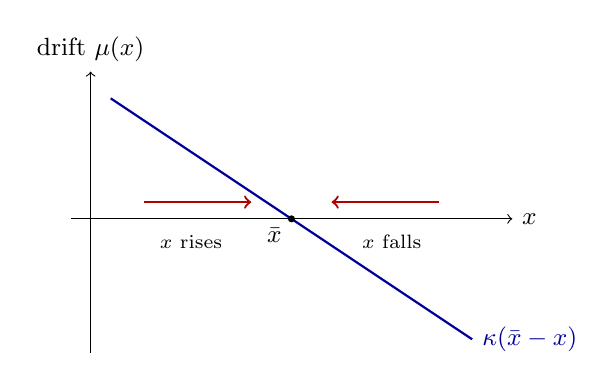
\begin{tikzpicture}[scale=0.85,every node/.style={font=\small}]
\draw[->] (-0.3,0)--(6.3,0) node[right]{$x$};
\draw[->] (0,-2)--(0,2.2) node[above]{drift $\mu(x)$};
\draw[thick,blue!60!black] (0.3,1.8)--(5.7,-1.8) node[right]{$\kappa(\bar x-x)$};
\fill (3,0) circle (1.5pt) node[below left]{$\bar x$};
\draw[->,thick,red!70!black] (0.8,0.25)--(2.4,0.25);
\draw[->,thick,red!70!black] (5.2,0.25)--(3.6,0.25);
\node[font=\scriptsize] at (1.5,-0.35) {$x$ rises};
\node[font=\scriptsize] at (4.5,-0.35) {$x$ falls};
\end{tikzpicture}
\end{center}
\textit{How to read the figure.} The horizontal axis is the current value of $x$; the vertical axis is the drift (expected change per unit of time). The drift line slopes down with slope $-\kappa$ and crosses zero at $\bar x$. To the left of $\bar x$ the drift is positive, so $x$ tends to rise; to the right it is negative, so $x$ tends to fall (red arrows). A steeper line (larger $\kappa$) means faster mean reversion.

\paragraph{Geometric Brownian motion (GBM).} $\mu(x,t)=\mu x$, $\sigma(x,t)=\sigma x$:
\begin{equation}\label{eq:gbm}
dx_t=\mu x_t\,dt+\sigma x_t\,dW_t\qquad\Longleftrightarrow\qquad \frac{dx_t}{x_t}=\mu\,dt+\sigma\,dW_t.
\end{equation}
\begin{itemize}
\item $\mu$ is the expected growth rate of $x$ and $\sigma$ the volatility of its growth rate.
\item The variance of $dx$ is not constant: it is $\sigma^2x^2dt$, proportional to the level of $x$ squared.
\item $x_t>0$ for all $t$ if $x_0>0$. Using It\^o's lemma (Example 2 below), $x_t=x_0\exp\!\big((\mu-\tfrac12\sigma^2)t+\sigma W_t\big)$, so $\log x_t$ is an arithmetic BM and $x_t$ is log-normal with $\mathbb{E}[x_t]=x_0e^{\mu t}$.
\end{itemize}

\subsubsection{Standard vs.\ general BM; BM vs.\ GBM}
\begin{itemize}
\item \textbf{Standard BM:} $W_0=0$ and independent increments $W_{t_2}-W_{t_1}\sim N(0,t_2-t_1)$; in discrete steps $W_t=W_{t-\Delta t}+\varepsilon\sqrt{\Delta t}$, so it is centred at 0.
\item \textbf{General (arithmetic) BM:} has a drift, so it is not centred at 0 (its mean is $x_0+\mu t$). With constant $\mu,\sigma$ its increments are still stationary and independent: $x_t-x_s\sim N\big(\mu(t-s),\sigma^2(t-s)\big)$; and the underlying shock is still $dW_t\sim N(0,dt)$.
\item \textbf{BM = additive shocks:} the size of a shock does not depend on the level of $x$ (e.g.\ labour income).
\item \textbf{GBM = multiplicative shocks:} shocks are proportional to the level of $x$ (e.g.\ investment / capital income: a return shock hits each unit of wealth). This is why capital in the stochastic AK model follows a GBM.
\end{itemize}

%=====================================================================
\subsection{It\^o's lemma \pg{16--17}}\label{sec:ito}

\paragraph{Setup.} $x_t$ follows the diffusion $dx_t=\mu(x,t)\,dt+\sigma(x,t)\,dW_t$, which in integral form reads
\[
x_t=x_0+\int_0^t\mu(x_s,s)\,ds+\int_0^t\sigma(x_s,s)\,dW_s,
\]
where the last term is an It\^o integral. Let $y=f(x,t)$ be a smooth function. Question: given the SDE for $x$, what is the SDE for $y$?

\paragraph{Derivation.} Take a second-order Taylor expansion of $f$:
\[
dy=f_x\,dx+f_t\,dt+\tfrac12f_{xx}(dx)^2+f_{xt}\,dx\,dt+\tfrac12f_{tt}(dt)^2+\dots
\]
In ordinary calculus only first-order terms survive. Here, because $dW=\varepsilon\sqrt{dt}$, the term $(dx)^2$ contains $(dW)^2$, which is of order $dt$ and must be kept. Use the multiplication rules
\[
(dt)^2=0,\qquad dt\cdot dW=0,\qquad (dW)^2=dt
\]
(the first two are of order $dt^{3/2}$ or $dt^2$, negligible relative to $dt$). Then
\begin{align*}
(dx)^2&=\mu^2(dt)^2+2\mu\sigma\,dt\,dW+\sigma^2(dW)^2\qquad\text{(expand the square)}\\
&=0+0+\sigma^2dt=\sigma^2dt,
\end{align*}
and $dx\,dt=0$, $(dt)^2=0$.

\begin{keybox}[title=It\^o's lemma]
\[
dy=\frac{\partial y}{\partial x}dx+\frac{\partial y}{\partial t}dt+\frac12\frac{\partial^2y}{\partial x^2}(dx)^2,
\]
and after substituting $dx$ and $(dx)^2=\sigma^2dt$:
\begin{equation}\label{eq:ito}
dy=\Big(\mu f_x+f_t+\tfrac12\sigma^2f_{xx}\Big)dt+\sigma f_x\,dW.
\end{equation}
Two variables $g(x,y)$:
\[
dg=g_x\,dx+g_y\,dy+\tfrac12g_{xx}(dx)^2+\tfrac12g_{yy}(dy)^2+g_{xy}\,dx\,dy.
\]
\end{keybox}
\textit{Interpretation.} Compared with the ordinary chain rule, the drift of $y$ has an extra term $\tfrac12\sigma^2f_{xx}$: if $f$ is convex, volatility raises the expected change of $y$; if concave, it lowers it (Jensen's inequality).

\begin{tipbox}
Shortcut: when computing $(dx)^2$, square only the $dW$ term; everything with $dt$ drops out.
\end{tipbox}

\paragraph{Example 1: $y=e^x$ with $dx=\mu\,dt+\sigma\,dW$ (arithmetic BM).}
Derivatives: $\dfrac{\partial y}{\partial x}=e^x$, $\dfrac{\partial y}{\partial t}=0$, $\dfrac{\partial^2y}{\partial x^2}=e^x$; and $(dx)^2=\sigma^2dt$.
\begin{align*}
dy&=e^x\,dx+0\cdot dt+\tfrac12e^x(dx)^2\qquad\text{(It\^o's lemma)}\\
&=e^x(\mu\,dt+\sigma\,dW)+\tfrac12e^x\sigma^2dt\qquad\text{(substitute $dx$ and $(dx)^2$)}\\
&=e^x\mu\,dt+e^x\sigma\,dW+\tfrac12e^x\sigma^2dt\\
&=\Big(e^x\mu+\tfrac12\sigma^2e^x\Big)dt+e^x\sigma\,dW\qquad\text{(collect $dt$ terms)}\\
&=\Big(\mu+\tfrac12\sigma^2\Big)y\,dt+\sigma y\,dW\qquad\text{(use $e^x=y$)}.
\end{align*}
So $y=e^x$ is a GBM with growth rate $\mu+\tfrac12\sigma^2>\mu$: because $e^x$ is convex, the volatility of $x$ raises the expected growth of $y$.

\paragraph{Example 2: $y=\log x$.} Derivatives: $y_x=1/x$, $y_{xx}=-1/x^2$, $y_t=0$. Intuitively, since $\log$ is concave, $y$ grows more slowly than the naive guess.

\emph{(a) With $dx=\mu\,dt+\sigma\,dW$ (arithmetic BM):} $(dx)^2=\sigma^2dt$, so
\begin{align*}
dy&=\frac1x(\mu\,dt+\sigma\,dW)-\frac12\frac{1}{x^2}\sigma^2dt\\
&=\Big(\frac{\mu}{x}-\frac{\sigma^2}{2x^2}\Big)dt+\frac{\sigma}{x}\,dW.
\end{align*}
\emph{(b) With GBM $dx=\mu x\,dt+\sigma x\,dW$ (the usual case):} now $(dx)^2=\sigma^2x^2dt$, so
\begin{align*}
dy&=\frac1x(\mu x\,dt+\sigma x\,dW)-\frac12\frac{1}{x^2}\sigma^2x^2dt\\
&=\mu\,dt+\sigma\,dW-\tfrac12\sigma^2dt\\
&=\Big(\mu-\tfrac12\sigma^2\Big)dt+\sigma\,dW.
\end{align*}
\begin{keybox}[title=Log of a GBM]
$d\log x_t=\big(\mu-\tfrac12\sigma^2\big)dt+\sigma\,dW_t$, an arithmetic BM. Integrating from $0$ to $t$: $\log x_t=\log x_0+(\mu-\tfrac12\sigma^2)t+\sigma W_t$, i.e.\ $x_t=x_0\exp\!\big((\mu-\tfrac12\sigma^2)t+\sigma W_t\big)$.
\end{keybox}
The mean growth rate of $x$ is $\mu$, but the growth rate of $\log x$ (the median/typical path) is lower by $\tfrac12\sigma^2$.

\paragraph{Example 3: product of two correlated GBMs.}
\textit{Setup.}
\[
dx=\mu_1x\,dt+\sigma_1x\,dW_1,\qquad dy=\mu_2y\,dt+\sigma_2y\,dW_2,\qquad dW_2=\rho\,dW_1+\sqrt{1-\rho^2}\,dZ,
\]
where $W_1$ and $Z$ are two uncorrelated SBMs and $\rho\in[-1,1]$ is the correlation between $dW_1$ and $dW_2$ (here $\rho$ is a correlation, not the discount rate). Find $dg$ for $g=xy$.

\textit{Step 1: derivatives.} $g_x=y$, $g_y=x$, $g_{xx}=0$, $g_{yy}=0$, $g_{xy}=1$.

\textit{Step 2: the cross term.} Using $(dW_1)^2=dt$ and $dW_1\,dZ=0$ (uncorrelated), and dropping all products involving $dt$:
\begin{align*}
dx\,dy&=\sigma_1\sigma_2\,xy\,dW_1\,dW_2\\
&=\sigma_1\sigma_2\,xy\,dW_1\big(\rho\,dW_1+\sqrt{1-\rho^2}\,dZ\big)\\
&=\sigma_1\sigma_2\,xy\,\big(\rho\,dt+0\big)=\rho\,\sigma_1\sigma_2\,g\,dt.
\end{align*}
\textit{Step 3: apply the two-variable It\^o formula.}
\begin{align*}
dg&=y\,dx+x\,dy+\tfrac12\cdot0\cdot(dx)^2+\tfrac12\cdot0\cdot(dy)^2+1\cdot dx\,dy\\
&=y(\mu_1x\,dt+\sigma_1x\,dW_1)+x(\mu_2y\,dt+\sigma_2y\,dW_2)+\rho\sigma_1\sigma_2\,xy\,dt\\
&=(\mu_1+\mu_2+\rho\sigma_1\sigma_2)\,g\,dt+\sigma_1g\,dW_1+\sigma_2g\,dW_2.
\end{align*}
\textit{Step 4: volatility of $g$.} The shock term $\sigma_1\,dW_1+\sigma_2\,dW_2$ has variance per unit of time
$\sigma_1^2+\sigma_2^2+2\rho\sigma_1\sigma_2$ (variance of a sum with covariance $\rho\sigma_1\sigma_2$).

\begin{keybox}[title=Takeaways]
The product of two GBMs is again a GBM, with
\[
\frac{dg}{g}=(\mu_1+\mu_2+\rho\sigma_1\sigma_2)\,dt+\sigma_g\,d\widetilde W,\qquad \sigma_g=\sqrt{\sigma_1^2+\sigma_2^2+2\rho\sigma_1\sigma_2},
\]
where $\widetilde W$ is an SBM. Similarly, the sum of arithmetic (additive) BMs is again an arithmetic BM.
\end{keybox}
\textit{Interpretation.} The drift of the product is not just $\mu_1+\mu_2$: positive correlation ($\rho>0$) adds $\rho\sigma_1\sigma_2$, because when $x$ is high $y$ also tends to be high. Check via logs: $d\log g=d\log x+d\log y$ has drift $\mu_1+\mu_2-\tfrac12(\sigma_1^2+\sigma_2^2)$, which equals $\mu_g-\tfrac12\sigma_g^2$ with $\mu_g=\mu_1+\mu_2+\rho\sigma_1\sigma_2$, as it must.

%=====================================================================
\subsection{Markov chains: transition matrix and stationary distribution \pg{70}}

\paragraph{Setup (HW Q3).}
\begin{itemize}
\item $\lambda_t$: gross growth rate of the economy; it takes two values: bad state $\lambda_1=0.98$ (output shrinks 2\%), good state $\lambda_2=1.03$ (output grows 3\%).
\item $\lambda_t$ follows a (first-order) \emph{Markov chain}: the probability distribution of $\lambda_{t+1}$ depends only on the current state $\lambda_t$, not on earlier history.
\item $p_{ij}=\Pr(\lambda_{t+1}=\lambda_j\mid\lambda_t=\lambda_i)$: transition probabilities, collected in the \emph{transition matrix} $P$ (rows = today's state, columns = tomorrow's state; each row sums to 1).
\item $\pi_i$: long-run (stationary) probability of being in state $i$.
\end{itemize}
\[
P=\begin{bmatrix}p_{11}&1-p_{11}\\1-p_{22}&p_{22}\end{bmatrix}=\begin{bmatrix}0.8&0.2\\0.15&0.85\end{bmatrix}.
\]

\begin{center}
\begin{tikzpicture}[every node/.style={font=\small},>=Stealth]
\node[draw,circle,minimum size=1.3cm,align=center] (s1) at (0,0) {bad\\$0.98$};
\node[draw,circle,minimum size=1.3cm,align=center] (s2) at (4,0) {good\\$1.03$};
\draw[->,thick] (s1) to[bend left=25] node[above]{$1-p_{11}=0.2$} (s2);
\draw[->,thick] (s2) to[bend left=25] node[below]{$1-p_{22}=0.15$} (s1);
\draw[->,thick] (s1) to[loop left] node[left]{$p_{11}=0.8$} (s1);
\draw[->,thick] (s2) to[loop right] node[right]{$p_{22}=0.85$} (s2);
\end{tikzpicture}
\end{center}
\textit{How to read the figure.} Each circle is a state. An arrow from state $i$ to state $j$ carries the probability of moving from $i$ today to $j$ tomorrow; self-loops are the probabilities of staying. The probabilities on the arrows leaving any state sum to 1 (one row of $P$).

\paragraph{Reading the matrix.}
\begin{itemize}
\item If today we are in state 1 ($\lambda_t=0.98$): stay in state 1 with probability $p_{11}=0.8$; move to state 2 ($\lambda_{t+1}=1.03$) with probability $0.2$.
\item If today we are in state 2 ($\lambda_t=1.03$): stay in state 2 with probability $p_{22}=0.85$; move to state 1 ($\lambda_{t+1}=0.98$) with probability $0.15$.
\end{itemize}
Conditional expectations of next period's growth:
\begin{align*}
\mathbb{E}[\lambda_{t+1}\mid\lambda_t=0.98]&=0.8(0.98)+0.2(1.03)=0.784+0.206=0.990,\\
\mathbb{E}[\lambda_{t+1}\mid\lambda_t=1.03]&=0.15(0.98)+0.85(1.03)=0.147+0.8755=1.0225.
\end{align*}
Expected duration of a spell in state $i$ is $1/(1-p_{ii})$: $1/0.2=5$ periods for the bad state, $1/0.15\approx6.67$ periods for the good state.

\paragraph{Stationary distribution.} The goal is the unconditional mean $\mathbb{E}[\lambda]=\pi_1\lambda_1+\pi_2\lambda_2$, which requires the long-run probabilities $\pi=(\pi_1,\pi_2)$ (a row vector). Stationarity means that if today's state distribution is $\pi$, tomorrow's is also $\pi$:
\[
\pi=\pi P,\qquad \pi_1+\pi_2=1.
\]
Written out (probability of being in state $j$ tomorrow = sum over today's states of ``probability of being there'' times ``probability of moving to $j$''):
\begin{align}
\pi_1&=\pi_1p_{11}+\pi_2(1-p_{22}),\label{eq:mc1}\\
\pi_2&=\pi_1(1-p_{11})+\pi_2p_{22}.\label{eq:mc2}
\end{align}
Equations \eqref{eq:mc1} and \eqref{eq:mc2} are the same condition (adding them gives $\pi_1+\pi_2=\pi_1+\pi_2$), so we use one of them together with the adding-up constraint.

\textit{Step 1: rearrange \eqref{eq:mc1}.}
\begin{align*}
\pi_1-\pi_1p_{11}&=\pi_2(1-p_{22})\qquad\text{(move $\pi_1p_{11}$ to the left)}\\
\pi_1(1-p_{11})&=\pi_2(1-p_{22})\qquad\text{(flow out of state 1 = flow into state 1)}\\
\pi_2&=\frac{1-p_{11}}{1-p_{22}}\,\pi_1.
\end{align*}
\textit{Step 2: use $\pi_1+\pi_2=1$.}
\begin{align*}
\pi_1\Big(1+\frac{1-p_{11}}{1-p_{22}}\Big)&=1\\
\pi_1\,\frac{(1-p_{22})+(1-p_{11})}{1-p_{22}}&=1\\
\pi_1&=\frac{1-p_{22}}{2-p_{11}-p_{22}},\qquad \pi_2=1-\pi_1=\frac{1-p_{11}}{2-p_{11}-p_{22}}.
\end{align*}
\textit{Step 3: plug in the numbers.} $2-p_{11}-p_{22}=2-0.8-0.85=0.35$, so
\[
\pi_1=\frac{0.15}{0.35}=\frac37\approx0.4286,\qquad \pi_2=\frac{0.2}{0.35}=\frac47\approx0.5714.
\]
\textit{Check:} first column of $\pi P$: $\tfrac37(0.8)+\tfrac47(0.15)=\tfrac{2.4+0.6}{7}=\tfrac37=\pi_1$. \checkmark

\textit{Step 4: unconditional mean growth.}
\[
\mathbb{E}[\lambda]=\pi_1\lambda_1+\pi_2\lambda_2=\frac37(0.98)+\frac47(1.03)=\frac{2.94+4.12}{7}=\frac{7.06}{7}\approx1.0086.
\]

\begin{keybox}[title=Two-state Markov chain]
\[
\pi_1=\frac{1-p_{22}}{2-p_{11}-p_{22}},\qquad \pi_2=\frac{1-p_{11}}{2-p_{11}-p_{22}}.
\]
In HW Q3: $\pi=(3/7,\,4/7)$ and $\mathbb{E}[\lambda]\approx1.0086$, i.e.\ average growth of about $0.86\%$ per period.
\end{keybox}
\textit{Interpretation.} In the long run the economy spends more time in the good state because the good state is more persistent ($p_{22}=0.85>p_{11}=0.8$): the probability of leaving it is smaller. Each $\pi_i$ is proportional to the probability of \emph{leaving the other state}. Starting from any initial state, the rows of $P^n$ converge to $\pi$ as $n\to\infty$; the speed of convergence is governed by the second eigenvalue of $P$, $p_{11}+p_{22}-1=0.65$ (which is also the first-order autocorrelation of $\lambda_t$).
